%%%% OPTION
%% Change class according to your needs
%%  - article (no chapter)
%%  - report
%%  - etc.
\documentclass{report}


\IfFileExists{ifxetex.sty}{%
  \usepackage{ifxetex}%
}{%
  \newif\ifxetex
  \xetexfalse
}
  \ifxetex

\usepackage{fontspec}
\usepackage{xltxtra}
\setmainfont{DejaVu Serif}
\setsansfont{DejaVu Sans}
\setmonofont{DejaVu Sans Mono}
\else
\usepackage[T1]{fontenc}
\usepackage[latin1]{inputenc}
\fi
\usepackage{fancybox}
\usepackage{makeidx}
\usepackage{cmap}
\usepackage{url}
\usepackage{eurosym}
\usepackage{graphicx}

\usepackage[hyperlink]{sysfera}



%%%%
%% TODO:
%%  - ajouter une macro pour mettre l'objet du document
%%  - faire les footers avec l'adresse et tels de SysFera
%%  - enlever un max de paquets docbook


%%%%%%%%%%%%%%%%%%%%%%%%%%%%%%%%%%%%%%%%%%%%%%%%%%%%%%%%%%%%%%%%%%%%%%
%                            CONFIGURATION                           %
%%%%%%%%%%%%%%%%%%%%%%%%%%%%%%%%%%%%%%%%%%%%%%%%%%%%%%%%%%%%%%%%%%%%%%
% Use the following macros to configure your document
%%%%%%%%%%%%%%%%%%%%%%%%%%%%%%%%%%%%%%%%%%%%%%%%%%%%%%%%%%%%%%%%%%%%%%
%%%% OPTION
%% Change language: fr/en
%%  - for French: use french in babel, and fr in \setupsysferalocale
%%  - for English: use english in babel, and en in \setupsysferalocale
\usepackage[english]{babel}
\setupsysferalocale{en}

%%%% OPTION
%% Title and author of the document
\title{New approach of the forwarder architecture}
\author{K. COULOMB}

%%%% OPTION
%% Document reference
%% Use command \SFdocumentreference to set the document reference.
%% Latter on, you can use the \SFthisdocument macro to retrieve
%% this reference.
\SFdocumentreference{libdadiCORBA}
\SFprojectname{libdadiCORBA}
\SFprojectleader{B. DEPARDON}
%\SFclient{God}


%%%% OPTION
%% Release information. If the argument is not empty, then a box with
%% the content of the argument will be visible at the top of the document
%\SFreleaseinfo{} % will show "Travail en cours" at the
                                 % top of the page
%\SFreleaseinfo{} % won't show anything

%%%% OPTION
%% Draft watermark. You can also show a grey watermak on all pages of
%% your document using the following command.
%\showwatermark{DRAFT}

%%%% OPTION
%% Collaborators:
%% You can redefine the Indexation of the document using the following command:
% \renewcommand{\SFindexation}{
%   \begin{SFindtable}
%     \SFinditem{\writtenby}{Author 1}{06/06/2011}
%     \SFinditem{\correctedby}{Author 2}{22/07/2011}
%     \SFinditem{\validatedby}{Anonymous guy}{\date}
%   \end{SFindtable}
% }
% \renewcommand{\SFindexation}{} % disable this table


%%%% OPTION
%% Revision History Table:
%% Add a new \SFrevitem entry for adding a new entry in the revision
%% history table. Revision versions are added automatically.
\renewcommand{\SFrevhistory}{
\begin{SFrevtable}
  \SFrevitem{0.1}{05/01/2012}{First draft of the document}{K. COULOMB}
\end{SFrevtable}
}
% \renewcommand{\SFrevhistory}{} % disable this table


%%%% OPTION
%% References Table
%% Add a new \SFrefitem entry for adding a new entry in the list of
%% reference documents.
\renewcommand{\SFreferenceTable}{
\begin{SFreftable}
\end{SFreftable}
}
\renewcommand{\SFreferenceTable}{} % disable this table

%%%% OPTION
%% Authorization Table
%% Add a new \SFauthviewitem entry for adding a new entry in the list of
%% authorized users.
\renewcommand{\SFauthview}{
\begin{SFauthviewtable}
  \SFauthviewitem{SysFera}{tech@sysfera.com}
  \SFauthviewitem{Universit\'e Amiens}{Gael LE MAHEC}
\end{SFauthviewtable}
}
% \renewcommand{\SFauthview}{} % disable this table
%%%%%%%%%%%%%%%%%%%%%%%%%%%%%%%%%%%%%%%%%%%%%%%%%%%%%%%%%%%%%%%%%%%%%%
%                           /CONFIGURATION                           %
%%%%%%%%%%%%%%%%%%%%%%%%%%%%%%%%%%%%%%%%%%%%%%%%%%%%%%%%%%%%%%%%%%%%%%


\makeindex
\makeglossary


\begin{document}

\frontmatter % do not disable, this is used for page numbering
\maketitle % do not disable, otherwise you won't have any title
%%%% OPTION
%\tableofcontents % comment to disable the table of contents
\mainmatter % do not disable, this is used for page numbering


%%%%%%%%%%%%%%%%%%%%%%%%%%%%%%%%%%%%%%%%%%%%%%%%%%%%%%%%%%%%%%%%%%%%%%
%              Write your document below this comment                %
%%%%%%%%%%%%%%%%%%%%%%%%%%%%%%%%%%%%%%%%%%%%%%%%%%%%%%%%%%%%%%%%%%%%%%

\chapter*{Introduction}

% \href{mailto:mail@exemple.com}{Mon mail} % Lien email
% \href{http://exemple.com}{Mon site web}  % Lien web
% \href{fichier.pdf}{Mon fichier}          % Lien vers un fichier
%\Acrobatmenu{FullScreen}{Plein écran}    % Plein écran/fenêtré

In a distributed application, the communication layer is an important tool. It
enables different objects to communicate. The problem is that various elements
may be located in different domains, or isolated by firewalls. The aim of the 
libdadiCORBA library is to provide a CORBA layer that can pass throught the 
firewall. The libdadiCORBA offers a mechanism that, if one has IDLs, he adds 
them to the library and create the forwarder version (along with their 
implementation) and can then go throught the forwarder to reach various domains.

\chapter*{forwarders}
\label{ch:forwarders}
The libdadiCORBA middleware uses CORBA as its communication layer. It is an easy
and flexible way for the different platform components to communicate.
However, deploying on heterogeneous networks that are not
reachable from each other except through ssh connection is a complicated
task needing complex configuration. Moreover, to ensure that all
objects can contact each others, we need to set-up and launch ssh
tunnels between eaceh of them, reducing significantly the
scalability in that network configuration context.

The \textit{forwarders} are the solution for such a situation, by
reducing the number of ssh tunnels to the minimum and making their
launch totally transparent for the final users. The forwarders
configuration is very simple even for very complex network topologies.

The next section presents the global operation of
forwarders. Section \ref{sec:ForwarderConfig} presents the forwarder
executable, its command-line options and configuration file. Then,
section \ref{sec:ForwarderExamples} gives two examples of forwarder
configurations.

\section*{Easy CORBA objects connections through ssh}
Each CORBA object in is reachable through omniORB using a TCP
port and the hostname of the machine on which it is executed. By
default these parameters are fixed automatically by omniORB but it is
also possible to choose them statically using the SysFera-DS configuration
file.
When two objects are located on different networks that are reachable
only through ssh, it is easy to open an ssh tunnel to redirect the
communications between them on the good port and host. Then, correcting
the objects bindings into the omniNames servers is sufficient to ensure
the communications between the different objects. To allow two
CORBA objects to communicate through an ssh tunnel, users must:
\begin{itemize}
\item Start the process which declares the objects and register them
  into the omniNames server(s).
\item Open ssh tunnels that redirect the local objects ports to
  remote ports.
\item Modify the objects bindings in the omniNames server(s) to make
  them point to the forwarded ports.
\end{itemize}

When using few objects that do not need much interaction, these steps
can easily be done ``manually''. But libdadiCORBA uses several different
objects for each element and is designed to manage thousands of nodes.
Moreover, creating an ssh tunnel between all the nodes of a Grid
cannot even be considered.

The forwarders deal with this problem by creating \textit{proxy
  objects} that forward the communications to a peer forwarder through
a unique ssh tunnel. Then, only one ssh tunnel is created to connect
two different networks. This system also allows users to define complex
communications routing. Figure \ref{fig:forwarder} shows how the
forwarders work to route communications through ssh tunnels. Moreover
most of the configuration of the forwarders automatically can be set
by itself.

\begin{figure}[htp]
\begin{center}
  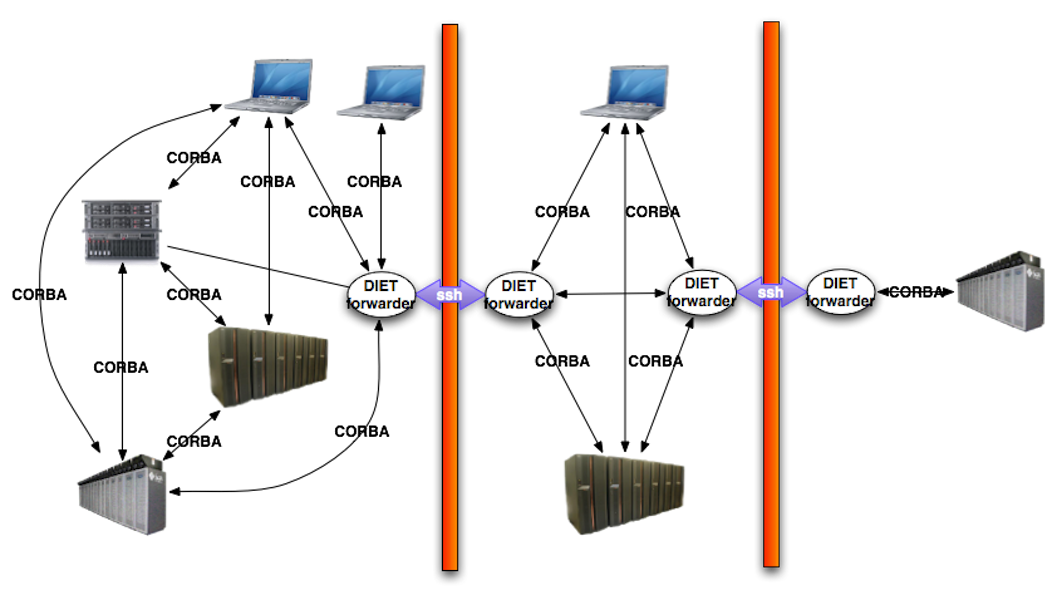
\includegraphics[width=12cm]{fig/Forwarder}
\end{center}
\caption{Forwarders routing SysFera-DS communication through ssh tunnels
  \label{fig:forwarder}}
\end{figure}

\section*{The corbaForwarder executable}
\label{sec:ForwarderConfig}
An executable called \textit{corbaForwarder}
is installed on the \textit{bin} directory. It allows to launch a
forwarder object following the configuration passed on the command
line.
\subsection*{Command line options}
The corbaForwarder executable takes several options to be launched:
\begin{itemize}
\item \verb#--name#: to define the name of the forwarder.
\item \verb#--peer-name#: the name of its peer on the other network.
\item \verb#--ssh-host#: the ssh host for the tunnel creation.
\item \verb#--ssh-port#: the port to use to establish the ssh
  connection (by default: 22).
\item \verb#--ssh-login#: the login to use to establish the ssh
  connection (by default: current user login).
\item \verb#--ssh-key#: the private key to use to establish the ssh
  connection (by default: \verb#$HOME/.ssh/id_rsa#).
\item \verb#--remote-port#: the port to listen on the ssh host (by
  default: the remote forwarder tries to dermine an available port
  automatically, note that if the connection fails when you do not use
  this option, then you have to specify the remote port).
\item \verb#--remote-host#: the host to which the connection is made
  by the tunnel (corresponds to \verb#host# in the ssh options
  \verb#-L# and \verb#-R#).
\item \verb#--nb-retry#: the number of times the local forwarder tries
  to bind itself to the distant forwarder (default is 3).
\item \verb#--peer-ior#: if you already know the IOR of the distant
  forwarder, then you can pass it to your local forwarder. By default,
  the local forwarder retrieves the IOR of its peer.
\item \verb#--tunnel-wait#: the time is seconds that the forwarder
  will wait while opening the ssh tunnel.
\end{itemize}
The remote port can be chosen randomly among the available TCP ports
on the remote host. Sometimes, depending on the configuration of sshd,
you will need to set \verb#--remote-host# to \verb#localhost# or
\verb#127.0.0.1# (or the address of the local loopback if it is not
\verb#127.0.0.1#) for the tunnel to work correctly (in fact, most
problems come from a badly configured tunnel).\\

\noindent In order, to activate a forwarder, users must:
\begin{itemize}
\item Launch omniNames on the remote and local hosts.
\item Launch the first peer on the remote host, only defining its name
  and its network configuration.
\item Launch the second peer, passing it it the first peer name, the
  ssh connection informations, the remote port to use and its network
  configuration.
\end{itemize}


\section*{Configuration examples}
\label{sec:ForwarderExamples}

The first example presents the configurations of forwarders to
connect a SysFera-DS \sed located on a network only reachable through ssh to a
SysFera-DS hierarchy located on another network.\\

The second example presents the configurations of forwarders to
connect three networks: the first one can only reach the second one
through ssh and the third one can also only reach the second one
through ssh. We want to connect SysFera-DS elements distributed over the
three networks.

\subsection*{Simple configuration}
\begin{itemize}
\item The two different domains are \textit{net1} and \textit{net2}. The forwarders will
  be launched on the hosts \textit{fwd.net1} and \textit{fwd.net2}.
\item There is no possibility to access \textit{fwd.net1} from
  \textit{fwd.net2} but users can access \textit{fwd.net2} from
  \textit{fwd.net1} using an ssh connection.
\item The forwarder on \textit{fwd.net1} is named \textit{Fwd1}, the
  forwarder on \textit{fwd.net2} is named \textit{Fwd2}.
\item One \sed is launched on \textit{fwd.net2}, the rest of the Sysfera-DS
  hierarchy is launched on the \textit{net1} domain.\\
\end{itemize}

\noindent\textbf{Command line to launch \textit{Fwd1}: }\\
{\small \it fwd.net1\$ corbaForwarder {\tiny$--$}name Fwd1
  {\tiny$--$}peer-name Fwd2 $\backslash$\\
  \hspace*{4.2cm}{\tiny$--$}ssh-host fwd.net2 {\tiny$--$}ssh-login
  dietUser $\backslash$\\
  \hspace*{4.2cm}{\tiny$--$}ssh-key id\_rsa\_net2
  {\tiny$--$}remote-port 50000}\\[2mm]
\noindent\textbf{Command line to launch \textit{Fwd2}: }\\
{\small \it fwd.net2\$ corbaForwarder {\tiny$--$}name Fwd2}\\[3mm]

Note that \textit{Fwd2} has to be launched before \textit{Fwd1}.
When the two forwarders are launched, the user can deploy his SysFera-DS
hierarchy. All the communications through  forwarders are
transparent.

\subsection*{Complex network topology}
To connect the three domains, we need 4 forwarders (2 pairs): one on
\textit{net1}, two on \textit{net2} and one on \textit{net3}.
\begin{itemize}
\item The three domains are: \textit{net1}, \textit{net2} and
  \textit{net3}.
\item The machines located on \textit{net1} and \textit{net3} are only
  reachable from \textit{fwd.net2} through ssh.
\item The four forwarders are named \textit{Fwd1}, \textit{Fwd2-1},
  \textit{Fwd2-3} and \textit{Fwd3}.
\item The hierarchy is distributed on the three networks.\\
\end{itemize}

\noindent\textbf{Command line to launch \textit{Fwd1}: }\\
{\small \it fwd.net1\$ corbaForwarder {\tiny$--$}name Fwd1}\\[2mm]

\noindent\textbf{Command line to launch \textit{Fwd2-1}: }\\
{\small \it fwd.net2\$ corbaForwarder {\tiny$--$}name Fwd2-1
  {\tiny$--$}peer-name Fwd1 $\backslash$\\
  \hspace*{4.2cm}{\tiny$--$}ssh-host fwd.net1 {\tiny$--$}ssh-login
  dietUser $\backslash$\\
  \hspace*{4.2cm}{\tiny$--$}ssh-key id\_rsa\_net1
  {\tiny$--$}remote-port 50000}\\[2mm]

\noindent\textbf{Command line to launch \textit{Fwd2-3}: }\\
{\small \it fwd.net2\$ corbaForwarder {\tiny$--$}name Fwd2-3
  {\tiny$--$}peer-name Fwd3 $\backslash$\\
  \hspace*{4.2cm}{\tiny$--$}ssh-host fwd.net3 {\tiny$--$}ssh-login
  dietUser $\backslash$\\
  \hspace*{4.2cm}{\tiny$--$}ssh-key id\_rsa\_net3
  {\tiny$--$}remote-port 50000}\\[2mm]

\noindent\textbf{Command line to launch \textit{Fwd3}: }\\
{\small \it fwd.net3\$ corbaForwarder {\tiny$--$}name Fwd3}\\[3mm]

Using this configuration, a communication from a host on \textit{net1}
to a host on \textit{net3} is first routed from \textit{Fwd1} to
\textit{Fwd2-1} and then from \textit{Fwd2-3} to \textit{Fwd3}.
Note that \textit{Fwd1} has to be launched before \textit{Fwd2-1}, and
\textit{Fwd3} has to be launched before \textit{Fwd2-3}.

\end{document}
